\chapter{相关技术研究}
经典的知识图谱嵌入模型通过提取三元组中的事实特征来对实体和关系编码,并使用如TransE、RESCAL等模型设计的评分函数来对嵌入后的三元组进行打分,以改进图谱嵌入的效果。但在跨设备的知识图谱的应用场景下,图谱会引入训练数据中不存在的未见的实体和未见的关系,导致传统的嵌入模型无法学习到这些组件的特征表示。为了解决这一问题,研究者往往会借助除三元组之外的辅助信息来加强对未见组件的特征提取,比如实体的位置信息、邻接关系及图谱包含的其他文本信息等。由于这些信息与训练数据的没有很强的依赖关系,因此可以迁移到未见的组件上,从而学习出通用的特征来进行嵌入表示。然而,现存的相关模型为了摆脱数据强依赖的特性,在研究图谱中对未见组件编码进行特征表示时,忽略了知识图谱作为知识网络中包含的丰富的语义信息,没有很好进行多维度知识的融合。

% 为了改善这一问题,本文尝试在学习图谱中可迁移到未见组件的特征表示的过程中融合图谱高层语义信息的本体知识,同时采用元学习的训练方法来进行场景模拟和快速学习。本节将简要介绍涉及到的元学习训练方法和归纳、本体嵌入知识图谱嵌入模型的相关内容。

为了解决这一问题,本文探索了将本体知识融合到学习图谱中可迁移的特征表示的过程中,并采用元学习的训练方法对场景进行模拟和快速学习。本节将简要介绍涉及到的元学习训练方法和归纳、本体嵌入知识图谱嵌入模型的相关内容。

\section{知识图谱本体嵌入}
本体作为表示和交换通用或主要知识的载体,通常以层次概念作为描述语义关系的主干和属性,并且可以选择性地定义一些逻辑约束,例如类的不相交性、属性域和可取值的范围。随着知识图谱在知识问答、推荐系统等下游任务上的广泛应用,像NELL-995\cite{xiong2017deeppath}和DBpedia\cite{auer2007dbpedia}这样的几个大型的知识图谱在研究和实际应用中被广泛使用。这些经典知识图谱通常会被从两个方面进行使用:一方面从实例出发,这些知识图谱存储了丰富的事实三元组,每个三元组中的实体由关系进行连接,如(奥巴马,政治家,美国);而从本体的视角,知识图谱从广泛的事实三元组中进行提取构建抽象概念的语义元关系,如(政治家,领导,国家)。同时,知识图谱还能提供实体到本体的相关映射关系。这些存储在知识图谱中对知识的高高层抽象是对知识图谱语义结构的集中表示。

\begin{figure}
  \centering
  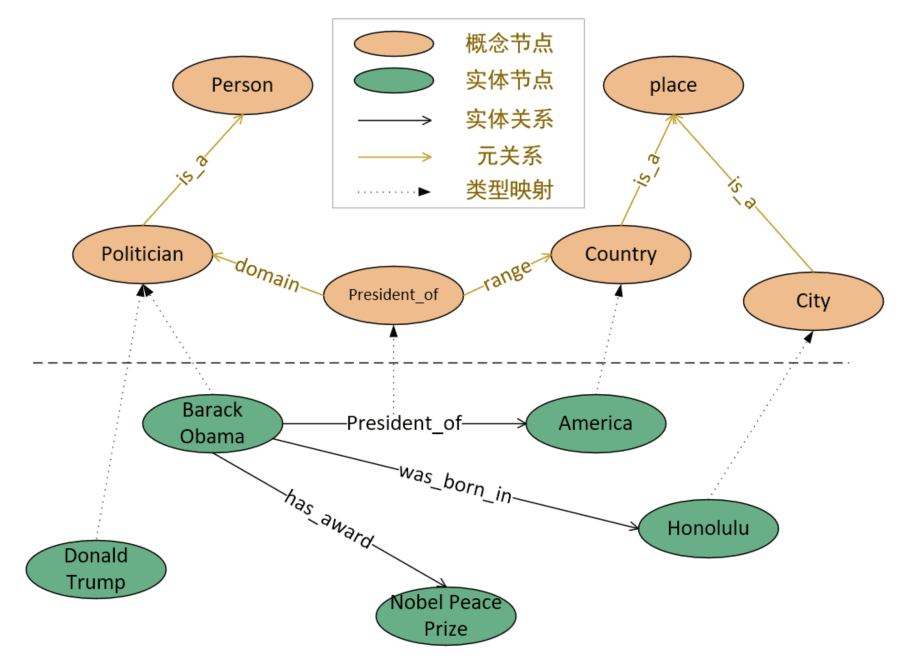
\includegraphics[width=0.6\textwidth]{2-1.png}
  \caption{知识图谱的本体视角和实例视角}
  \label{fig:2-1}
\end{figure}

在知识图谱表示学习中,基于翻译的模型和基于语义匹配的模型已经被广泛应用,并且在一定程度上取得了不错的效果。然而,这两种模型都有一些局限性,它们忽略了知识图谱中包含的额外知识。知识图谱中的实体往往有着不同的类型信息,这些信息可以帮助模型更好地理解实体之间的关系。基于翻译的模型和基于语义匹配的模型通常只考虑了实体本身的信息,而没有利用实体类型的信息。另外,知识图谱中的实体之间通常存在层次关系,例如子类和父类之间的关系,这些层次关系可以为模型提供更多的语义信息,但是这些信息没有被基于翻译的模型和基于语义匹配的模型都没有很好地利用。相反,利用这些全局信息进行表示的模型可以通过将语义或者结构信息整合到知识嵌入过程中来增强知识表示的学习效果。

一些利用本体进行知识图谱表示学习的方法将本体信息作为实体的额外类型信息,实体借用本体定义的更高层次的类型来表示,关系也使用语义类型进行表示。例如,将“马斯克”用本体定义的“人类”概念节点进行表示,“特斯拉”则被表示成所属的“公司”节点。这些简单的引入类型信息的方法是基于传统的基于三元组的模型的扩展,它集成了额外的文本信息来改进其性能。SSE\cite{guo2016sse}模型结合实体的语义类别,将属于同一类别的实体平滑地嵌入到语义空间中。为了能够更有效的捕捉到这些高层本体类型信息带来的限制效果,该模型提出了两种在语义层面对嵌入变量的限制。首先该模型通过拉普拉斯特征映射的算法思想认为同一个语义类别下的实体的嵌入应该更加相近,即“法国”实体和“意大利”的实体因为同属于国家的语义所以他们对应的嵌入表示应该更为相似。因此,模型为每一个实体设置了一个语义分类矩阵\(W^{(1)}_{ij}\),如果任意两个实体在类型上相同,那么该矩阵中对应的值即为1,否则为0,基于该矩阵计算两个实体之间的语义平滑值:
\begin{equation}
  \mathcal{R}_{1} = \frac{1}{2} \sum_{i=1}^{n} \sum_{j=1}^{n} \| e_{i} - e_{j} \|_{2}^{2}W^{(1)}_{ij} \label{eq:2-1}
\end{equation}

其中\(e_{i}\)和\(e_{j}\)指代两个实体i和实体j对应的嵌入表示,通过使得两个同类实体的语义平滑值最小来实现拉普拉斯特征映射的语义限制。其次该模型还提出基于局部线性嵌入的语义约束思想,不同于拉普拉斯特征映射的对数据对局部不变性的设定,基于局部线性嵌入的思想认为一个实体可以通过其最接近的邻居节点通过一个线性的组合器来近似的表征,举例如“法国”的实体嵌入可以通过其语义相邻的节点如“中国”、“意大利”等国家节点通过线性组合的方式来近似的表示。同样,在该语义约束下SSE设置了一个类别邻接矩阵\(W^{(2)}_{ij}\),该矩阵指明实体的连接节点是否是该节点语义范畴内的最邻近节点。然后在该约束下计算实体的语义平滑值:
\begin{equation}
  \mathcal{R}_{2} = \sum_{i=1}^{n} \left\| e_{i} - \sum_{e_{j}\in\mathcal{N}(e_{i})}W^{(2)}_{ij}e_{j} \right\|_{2}^{2} \label{eq:2-2}
\end{equation}

其中\(e_{i}\)和\(e_{j}\)指代两个实体i和实体j对应的嵌入表示,通过使得实体i和所有最邻近节点的线性组合距离最短来实现该猜想的约束。最后该模型分别通过在基于距离和基于语义相似度的嵌入模型上加入两种语义的约束来提高嵌入表示的效果。实验证明在高层语义类别的约束下的表示学习取得了很好的嵌入效果。虽然通过这两种类别信息的约束能够有效的引入了图谱除结构外额外的知识,但是该模型认为一个实体只属于一个类别,忽略了多个类别可能存在的联系,没有完全充分利用好高层的语义知识。

同样借助于本体的类型信息,JOIE\cite{hao2019universal}模型从本体和实例三元组两个不同的层次分别进行嵌入学习,设计了跨视图和视图内建模模型,从知识库的多个方面进行学习。一方面学习了跨视图关联模型,实现本体概念与相应实例视图实体之间的连接。另一方面对视图内模型进行训练,以在单独的嵌入空间中捕获实例视图和本体视图的结构化知识,并为具有层次结构的本体启用了层次感知编码技术,虽然这两个模型都运用到了本体的类型信息,但是他们也使用了单一的类型,没有充分考虑到本体丰富的其他语义关系。

TKRL\cite{xie2016representation-TKRL}模型基于传统的翻译模型并结合本体的实体类型信息提出了一个type-embedding的嵌入方法。与SSE模型实体单一类别的设定不同,TKRL模型认为一个实体可能有多个不同层次的类别,并且这些不同层次的类别信息应该被转化到与类别绑定的不同的特征空间中,因此三元组中的每个实体都应该包含多个实体类型相关的特征信息联合表示。而为了获取到实体的多类别的语义信息,TKRL模型采用所有实体类型转换矩阵的加权和来计算出最后的转换矩阵:
\begin{equation}
  M = \frac{\sum^{n}_{i = 1}\alpha_{i}M_{c_{i}}}{\sum^{n}_{i = 1}\alpha_{i}}, \alpha_{i} = \left \{\begin{array}{ll}
    1,\quad c_{i} \in C\\
    0,\quad c_{i} \notin C
    \end{array} 
    \right.\label{eq:2-3}
\end{equation}

其中n是一个实体所有可能的实体类型数量,指代第i个实体类型,是该实体类型对应的转化矩阵,是矩阵对应的权重值,最后的指代三元组给定三元组(h,r,t)头实体所有与关系r相连接的可能的实体类型的集合。TKRL引入实体类型并对所有可能的类型信息进行聚合来增强嵌入模型的学习效果。

为了提高知识表示学习的性能,现有的大多数本体模型在知识嵌入过程中都包含了单一的本体信息,无法实现对所有可用本体信息的无缝嵌入。在现实世界中,知识图谱通常是不完整的,单一的本体信息对补充图谱的作用是有限的。本文能够在知识嵌入过程中无缝地整合所有可用的本体信息,充分补充图谱,提高复杂场景下的决策能力。同时本文使用了一种简单的本体形式,即RDF Schema(RDFS)中,而那些更复杂的OWL本体可以按照一定的标准转换为RDFS本体。本体可以用作知识图谱的模式,定义实体类型、关系等。本文将本体集合表示为\(\mathcal{O} = \{\mathcal{C}, \mathcal{P},\mathcal{T}_{o}\}\),其中\(\mathcal{C}\)是概念节点的集合(即实体类型和实体关系),\(\mathcal{P}\)是属性的集合,\(\mathcal{T}_{o}\)是本体三元组的集合。

\section{归纳知识图谱表示学习}
随着知识图谱日益增多的落地应用,图谱在分布的终端上独立的更新和训练,越来越多的出现了类似训练集中不存在但现实中又遇到的实体或关系等出现未见组件的情况,为了能够更好的将模型适用于这种现实的场景需求,一些通过归纳推理的模型也取得了一定的效果。

为了弥补仅从实体三元组学习嵌入导致不适用于训练集中不可见的实体的弊端,一些研究者首先尝试了从用额外的知识对嵌入表示学习进行补充使得对未见组件的嵌入可以从额外的知识中学习出一定的有效特征。例如IKRL模型在首次在原有的实体三元组的基础上补充了视觉的信息,将头尾实体的图像信息作为图像特征进行编码并和三元组学习的特征进行融合,在知识图谱补全任务和三元组分裂任务上都取得了很好的效果。不同于传统的知识图谱都是固定的且实体基本上不不会随意新增的“closed-world”的知识图谱补全任务,ConMask\cite{shi2018open}为了解决知识图谱不断发展中很有可能出现的未见的实体提出了一种“open-world”下的表示学习方法。该模型了为了能够实现包含未见实体的知识图谱补全任务,将学习的重点转移到了实体的描述文本上,模型包含三个部分:首先通过目标关系的名称圈出和任务相关联的单词并抹去不想干的单词;然后从实体的名字和实体的描述文本中学习到该实体的嵌入表示;最后通过计算各候选实体与目标实体在任务上的相似度来判断是否能组成事实三元组。虽然上述的方法在响应的知识图谱补全任务上都取得了一定的效果,但是没有足够的证据表明这些方法能够判断出文本和图像中的隐含事实。同时在一些情况下,假设新实体并没有提供描述文本或者图像信息时可能这些方法的效果就会大打折扣。

除了引入实体或者关系的某一特定类型的信息作为对未见组件特征知识来源的方法外,一些研究者通过对现有信息学习出逻辑上的规则来进行归纳表示学习,这些方法通过在训练集上学习出的独立于实体节点的规则来覆盖到未见的实体上进行表示。传统的基于规则的表示学习方法如AMIE\cite{galarraga2013amie}模型往往采用统计度量或者固定的人工设定的模式进行规则的学习,但是无疑这些方法有存在无法扩展的问题并且缺乏足够的推理表征能力。而最近的出现的一些可微规则学习方法如Neural LP\cite{yang2017differentiable}模型和DURM\cite{sadeghian2019drum}模型通过端到端的方法学习规则逻辑,通过设计可微的逻辑规则学习模型并通过基于梯度的方法进行优化求解,但是这些方法不能解决知识图谱中缺边的问题同时处理不合理的规则候选方面存在不足。而不同于直接从事实三元组中学习逻辑规则的方法,一些方法利用子图隐式地表示逻辑规则。GraIL和TACT\cite{chen2021topology}通过对未见实体周围的封闭子图的学习逻辑规则,但是很显然随着实体邻居数目的指数增长,这些子图的规模可能会很庞大从而可能导致效率问题。

不同于引入额外知识及学习全局逻辑规则的方法,未见实体的已知邻居节点的特征也被视为归纳推理模型的一种新型的知识输入。为了能够处理在训练阶段未观察到的测试实体的问题,GNN模型通过聚合所有邻接节点中已知部分的特征来作为未见组件的特征,该模型提供了一种在图上很好的通过聚合邻接特征来进行学习的思路。此后基于图神经网络的归纳知识图谱表示方法开始成为另外一类主要的研究路线。GNN模型专门用于处理图数据,可以直接输入一个图网络并能够很容易的进行节点级别、边级别及图级别的预测任务,相比于CNN模型只能作用在具有相同结构的图像或者特定序列的语音和文字上,图数据没有固定的形式且邻居节点的也都是无序的,因此无法作用在复杂的知识图谱上,而GNN通过聚合和更新操作能够有效学习到图谱结构和节点特征的有效信息。

为了有效的学习到图的结构信息和节点的特征并对特征进行嵌入,GNN主要包含了两个部分:聚合函数和更新函数,聚合函数可以对排名的邻接节点的特征进行聚合,常用的操作包含sum、mean以及max等。一次聚合操作可以将节点邻近一跳的邻接点的信息进行提取,而GNN一般包含多层,每一层都会接受上一层的信息在此进行聚合和传递,因此n层聚合后传递的信息会包含n层邻接节点的结构信息以及节点本身的特征信息。每层的特征聚合输出公式基本如下:
\begin{equation}
  h_{v}^{k} = \sigma(W_{k} \sum \frac{h_{u}^{k-1}}{|N(v)|} + B_{k}h_{v}^{k-1}) \quad where \quad k = 1, ..., k-1 \label{eq:2-4}
\end{equation}

从公式中可以看出每层的信息包含了两个部分,首先\(W_{k}\sum\frac{h^{k-1}_{u}}{|N(v)|}\)代表了对邻接点的特征聚合操作,而后一部分则是上一层聚合特征与一个可学习的权重参数的乘积,最后该两部分的特征通过一个激活函数来进行更新从而完成该层的节点特征输出。但是在GNN模型中聚合操作并没有区分邻接节点的重要性而是简单的进行了池化操作。为了增加对邻接点的关注度的区分,受到注意力机制在基于序列的任务上的优秀表现,GAT(Graph Attention Networks)将该机制引入到图图卷积网络中用于对图数据中的节点进行分类。注意力机制的好处之一是它可以处理可变大小的输入,并且聚焦于输入中最相关的部分来进行决策,而且在其他如RNN等模型在加入自注意力机制后也取得了不小的模型提升,可以证明该机制足以构建强大的模型。因此GAT使用注意力机制来判别邻居节点,计算图中的每个节点的隐藏表示,通过在节点-邻居对之间进行并行高效的计算而且可以指定邻居的任意权重来应用于具有不同度数的图节点,且相关论文的实验结果表明这种机制的引入同样可以高效地作用于归纳学习问题用于处理存在未知的组件等任务。

基于GNN的另外一种改进的方向聚焦于对图结构关系表示的补充上,图卷积神经网络集中于对节点特征的聚合和更新表示,在信息传递的过程中图的关系结构仅仅用于指明邻接点,关系的特征并没有参与到节点的更新过程中。为了增加关系信息对节点的影响,R-GCN在每层节点特征计算的过程中引入了邻接点及它们的关系:
\begin{equation}
  h_{i}^{l+1} = \sigma \left( \sum_{r\in\mathcal{R}} \sum_{j\in\mathcal{N}_{i}^{r}} \frac{1}{c_{i,r}}W_{r}^{l}h_{j}^{l} + W_{0}^{l}h_{i}^{l}\right) \label{eq:2-5}
\end{equation}

与GNN对邻接点特征聚合的操作不同,R-GCN引入了关系特定的转换\(W_{r}^{l}h_{j}^{l}\),这种转换取决于边的类型和方向,\(c_{i,r}\)是问题相对应的归一化参数。为了确保第l层的节点表示可以受到相应层次的表示的影响,R-GCN在基础的图关系上为每个节点添加了一个自连接的特殊关系。如图\ref{fig:2-2}所示,在R-GCN中每层对一个实体节点(红色块表示)进行特征生成的过程中,首先从邻接点获取特征(蓝色块表示)并根据该节点与邻接节点的关系类型进行特征转换得到该种关系对应的表示(绿色块表示),其中关系类型分别由入关系、出关系以及自循环关系组成;然后将所有关系转换后的邻接节点信息进行累加求和并通过一个如ReLU的激活函数即可获得该节点本层的输出表示。相比于R-GCN,近期提出的CompGCN在R-GCN模型同时考虑关系特征和节点特征对图数据进行嵌入表示的基础上进一步引入了注意力机制,CompGCN针对每种边类型和方向分别进行了注意力计算以加强对重要信息的关注,而且在计算效率方面,它减少了每个节点的嵌入大小并减少了依赖于固定卷积核的计算量,因此更适合于大规模图数据。
\begin{figure}
  \centering
  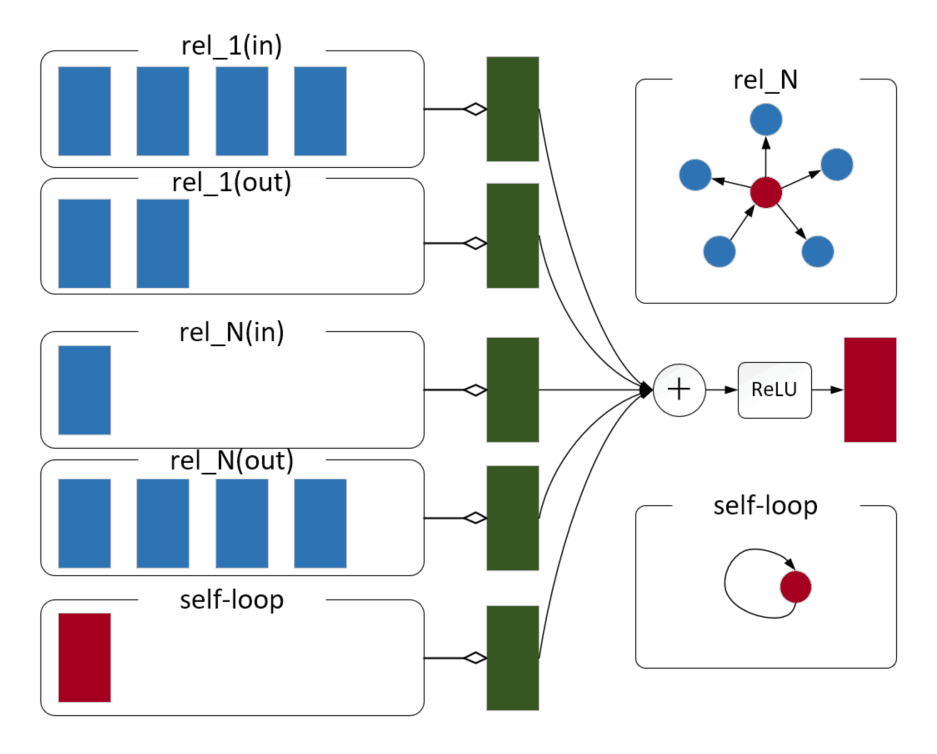
\includegraphics[width=0.8\textwidth]{2-2.png}
  \caption{R-GCN的特征传递}
  \label{fig:2-2}
\end{figure}

自图卷积网络广泛推广到图数据处理上后,其本身对于图数据隐藏知识的挖掘在一定程度上已经可以作用于归纳知识图谱表示学习上。近几年的归纳知识图谱表示学习的相关方法也大多利用图卷积神经网络进一步提升归纳表示学习的效果,例如INDIGO\cite{liu2021indigo}模型在GNN的基础上进行改进,使用实体三元组与GNN的最内层和最外层的特征向量元素之间的一对一对应关系对知识图谱进行编码。因此,预测的三元组可以直接从GNN的最后一层读出,而不需要额外打分函数,从而充分利用GNN的特征聚合能力。其他的相关的工作也有如xiong(2018)等人依赖邻域结构对未见关系进行编码学习的方法,但这些邻域的方法要么是专注于传统的知识图谱表示学习领域,要么是只能处理未见的关系而忽略未见的实体。本文通过本体全局信息的嵌入表示,可以同时对未见关系和位置实体进行辅助的嵌入表示,同时借助关系的位置结构信息加强知识的引入,从而训练处一个同时处理未见组件的归纳推理知识图谱表示学习模型。

\section{元学习训练方法}
学习最普适性的算法思想可以理解为learning to learn,它通过多个学习任务的训练来改进学习算法,而传统的机器学习算法则是在多个数据实例上进行模型的学习。

传统的机器学习方法会设置一个训练集\(\mathcal{D} = \{(x_{1},y_{1}),...,(x_{N},y_{N})\}\),例如样本对(输入的图片,图片的标签),本文的目的是训练出一个模型函数\(y = f_{\theta}(x)\),通过求解下述公式来获得其中的参数\(\theta\):
\begin{equation}
  \theta^{*} = \underset { \theta } { \operatorname { arg } \operatorname { min } }\mathcal{L}(\mathcal{D};\theta,w) \label{eq:2-6}
\end{equation}

% \begin{equation}
%   \mathcal{L}(\mathcal{T}_{que}^{i} | f_{\theta}(\mathcal{T}_{sup}^{i}), \theta)
% \end{equation}



其中的\(\mathcal{L}\)是一个损失函数来计算真实标签与模型预测标签之间的误差,指代了模型如何学习的假设,例如如何为参数\(\theta\)选择合适的优化器或者为选择函数类型等,传统的机器学习方法实现过程中该部分由研究者手动设置;而模型的泛化性能则通过评估该模型在已知标签上的测试集测试来衡量。传统的机器学习假设是模型的优化是对每个训练集\(\mathcal{D}\)从头开始执行,并且模型如何学习的相关设定\(w\)是预先指定好的。然而,模型如何学习的设定\(w\)会极大地影响到模型最后的准确性或数据效率等性能指标。元学习试图通过学习学习算法本身来改进这些指标,而不是假设学习算法是预先指定或者固定的。此外元学习从任务的分布中学习,而不是从头开始。

元学习learning to learn的思想精髓可以看做一个包含内外两层的双层优化问题,双层优化\cite{stackelberg1952theory}指代的是层次优化问题,其中一个优化包含另一个优化作为约束\cite{franceschi2018bilevel}\cite{sinha2017review}。经典的内外双层模型的算法如MAML,其算法流程如算法\ref{alg:meta}所示。

% \begin{algorithm}
%   \SetAlgoLined
%   \KwData{将训练集划分为子任务;初始化超参数}
%   随机初始化模型参数θ;\\
%   \While{未达到停止标准}{
%     从子任务中随机取batch\;
%     \For{所有batch}{
%       在batch上计算该任务的损失函数\;
%       基于损失函数使用少量的梯度下降更新参数\(\theta\)\;
%     }
%     计算各任务平均损失,采用梯度下降更新参数θ\;
%   }
%   \caption{Model-Agnostic Meta-Learing}\label{alg:alg1}
% \end{algorithm}

\begin{algorithm}
\KwData{\(p(\mathcal{T})\):distribution over tasks}
\KwData{\(\alpha,\beta\) step size hyperparameters}
  randomly initialize \(\theta\) \\
  \While{not done}{
  Sample batch of tasks \(\mathcal{T}_{i} \thicksim p(\mathcal{T})\)
  \For{\(\mathcal{T}_{i}\)}{
    Evaluate \(\nabla_{\theta}\mathcal{L}_{\mathcal{T}_{i}}(f_{\theta})\) wtih respect to K examples \\
    Compute adapted parameters with gradient descent:\(\theta^{'}_{i} = \theta - \alpha\nabla_{\theta}\mathcal{L}_{\mathcal{T}_{i}}(f_{\theta})\)
  }
  Update \(\theta \leftarrow \theta - \beta\nabla_{\theta} \sum_{\mathcal{T}_{i} \thicksim p(\mathcal{T})}\mathcal{L}_{\mathcal{T}_{i}}(f_{\theta^{'}})\)
}
\caption{Model-Agnostic Meta-Learing}\label{alg:meta}
\end{algorithm}

在该视角下,元学习任务可以通过如下公式来规范化:
\begin{equation}
  \omega ^ { * } = \underset { \omega } { \operatorname { arg } \operatorname { min } } \sum_{i=1}^{M} \mathcal{L} ^ { \text { meta } } ( \mathcal{D} _ { \text { source } } ^ { \text { val } ( i ) } ; \theta ^ { * ( i ) } , \omega ) \label{eq:2-7}
\end{equation}
\begin{equation}
  s.t. \qquad \theta ^ { * ( i ) } ( \omega ) = \underset { \theta } { \operatorname { arg } \operatorname { min } } \mathcal{L} ^ { \text { task } } ( \mathcal{D} _ { \text { source } } ^ { \text { train } ( i ) } ; \theta , \omega ) \label{eq:2-8}
\end{equation}

其中\(\mathcal{L} ^ { \text { meta } }\)和\(\mathcal{L} ^ { \text { task } }\)分别指代外层的优化目标和内层的优化目标,例如在分类任务下的交叉熵,但是这两层的优化级别并不对称,内层优化在基于外层参数\(\omega\)的优化过程中不能对\(\omega\)进行修改。而公式中\(\omega\)可以指代如非凸优化\cite{finn2017model}的内层模型的初始化参数或者内层模型的其他可学习的超参数。因此,元学习的整个训练流程分为了两层的优化:内层模型接收外层模型的参数\(\omega\),然后根据自己的任务对该任务的训练集进行训练并在任务的测试集上计算出损失函数;外层模型接收内层模型计算出的损失函数对参数\(\omega\)进行更新来使得内层函数的损失函数达到最优。元学习的思想即通过外层模型的训练学习到内层模型一个更好的设定,可以让内层模型更好的完成各种任务。

上面提到了内层模型在训练的时候需要针对面向的问题提供相应的训练集和测试集,这里的以任务为训练单位的设定也是元学习方法区别于传统机器学习方法的一大特点。从训练任务的角度来说,元学习的目标就是学习一种通用的能够作用在跨任务上的学习算法,这些学习到的算法能够在新的任务上获得更好的表现效果。内层模型可以视为带有外层模型参数\(\omega\)的经典的机器学习算法,其数据集 \(\mathcal{D} = (\mathcal{D}^{train}, \mathcal{D}^{val})\),针对单个任务的损失函数即为\(\mathcal{L}(\mathcal{D};\omega) = \mathcal{L}(\mathcal{D}^{val};\omega^{*}(\mathcal{D}^{train},\omega),\omega)\),而在实际应用中通常只有一个训练集和测试集,所以一般会从源训练集中抽样出一组用于训练的任务,在这些任务中的训练集和测试集为了避免和最终模型训练后进行评估的测试集混淆,一般称之为support集和query集。

元学习发展至今已经在许多领域展示出了它对推动当代深度学习行业前沿的巨大潜力,尤其是在深度学习领域饱受诟病的如数据效率问题、知识迁移问题以及无监督学习问题\cite{marcus2018deep}等方面展现出了更优秀的解决方案。在多任务场景,元学习已经证明可以从一系列任务中提取出来单个任务不可知的知识从而改进相关新任务的学习效果\cite{thrun1998learning};而在单任务场景下,元学习可以从该任务的重复处理中进行多个阶段的改进\cite{andrychowicz2016learning}\cite{liu2018darts}\cite{zhou2020online},也已成功应用在小样本图像识别\cite{snell2017prototypical}、数据效率提高\cite{houthooft2018evolved}和神经架构搜索(NAS)\cite{real2019regularized}等领域。而加利福尼亚大学的xiong等人(2018)\cite{xiong2018one}提出的工作是第一个针对知识图的少数镜头学习的研究。它是一种基于度量的模型,由相邻编码器和匹配处理器组成。邻居编码器通过实体的一跳邻居节点来增强实体的嵌入,匹配处理器通过LSTM块来实现多步匹配。

本文讨论跨领域跨设备的知识图谱上知识表示的相关研究并尝试解决在有未见组件的下游链接预测任务,经典的知识图谱表示学习的链接预测任务采用的数据集会设置一个训练集和测试集,测试集中不包含未见组件。因此,本文从现有数据集上采样出符合问题条件的数据,并借助于元学习learning to learn的思想,将这些数据打包为一个个任务,用于学习和训练,以期能够从这些数据中学习到能够处理未见组件的知识图谱表示。 